\section{定点数与浮点数}\label{sec:NumberSystemBasics/FixedPointAndFloatingPoint}
    解决了整数的二进制记录问题之后,我们需要考虑小数的记录的问题。

    我们可以参考在整数时使用的方式,直接记录小数的二进制,但是这会造成一个问题:由于二进制只有两个可用的记号 $0$ 和 $1$,而且它们都已经被用来表达数字,因此已经没有记号可以用来在数码之间标记出小数点的位置且不造成歧义。显然,“小数点在哪里”这个问题有两种解决方案,一种是事先约定好小数点的位置,一种是划出一段空间用来记录小数点的位置。

    \subsection{定点数}\label{subsec:NumberSystemBasics/FixedPointAndFloatingPoint/FixedPoint}
        对于一个有 $k$ 位的设备,如果我们事先约定小数点的位置在 $n$ 位与 $n + 1$ 位之间的话,那么这个小数的表达方式就能总结为如下几点:
        \begin{enumerate}
            \item 左起第一位为符号位;
            \item 左起第二位到第 $n$ 位是整数部分的二进制记录;
            \item 左起第 $n + 1$ 位到第 $k$ 位是小数部分的二进制记录。
        \end{enumerate}

        此时它可以表达的数的范围是 $(-\underbrace{11 \cdots 11}_{n-1}.\underbrace{11 \cdots 11}_{k-n})_2$ -- $(-0.\underbrace{00 \cdots 00}_{k-n}1)_2$ 和 $(0.\underbrace{00 \cdots 00}_{k-n}1)_2$ -- $(\underbrace{11 \cdots 11}_{n-1}.\underbrace{11 \cdots 11}_{k-n})_2$,或者说 $-\frac{2^{(k-1)}-1}{2^{(k-n)}}$ -- $-\frac{1}{2^{(k-n)}}$ 和 $\frac{1}{2^{(k-n)}}$ -- $\frac{2^{(k-1)}-1}{2^{(k-n)}}$,分度值为 $(0.\underbrace{00 \cdots 00}_{k-n}1)_2$,或者说 $\frac{1}{2^{(k-n)}}$。

        一个具体的例子如~\ref{tab:NumberSystemBasics/FixedPointAndFloatingPoint/FixedPoint/DataRange} 所示。

        % https://tex.stackexchange.com/a/130008/149813
        \begin{table}
            \centering
            \begin{tabular}{lS[table-format=-3.7]S[table-format=-3.7]S[table-format=-3.7]}
                $n$ & 最小值     & 最大值    & 分度值    \\ \hline
                1   & -0.9921875 & 0.9921875  & 0.0078125 \\
                2   & -1.984375  & 1.984375   & 0.015625  \\
                3   & -3.96875   & 3.96875    & 0.03125   \\
                4   & -7.9375    & 7.9375     & 0.0625    \\
                5   & -15.875    & 15.875     & 0.125     \\
                6   & -31.75     & 31.75      & 0.25      \\
                7   & -63.5      & 63.5       & 0.5       \\
                8   & -127       & 127        & 1         \\
            \end{tabular}
            \caption{$k = 8$ 时 $n$ 的值对应的数据范围}
            \label{tab:NumberSystemBasics/FixedPointAndFloatingPoint/FixedPoint/DataRange}
        \end{table}

        对于以上的定义,

        这种记录小数的方式,在一开始小数点的位置就被固定了,因此称为“定点数”(Fixed Point):比如说,对于二进制小数 $(100.11)_2$ 来说,不管如何修改 $k$ 和 $n$,这个数的小数点的位置总是在第二个 $0$ 和第二个 $1$ 之间,这个小数点的位置是固定不变的,这就是“定点数”一名的来源。

        然而,这种记录方式有一个问题:精度与范围只能二选一。如果使用更小的 $n$,精度就能提高,但是所能表达的数的范围便急剧减小;如果提升表达的数的范围,就需要使用更大的 $n$,这导致了精度的降低。如果我们将所使用的权重画出来,就会是如图~\ref{fig:NumberSystemBasics/FixedPointAndFloatingPoint/FixedPoint/Position} 所示的情况:

        \begin{figure}
            \centering
            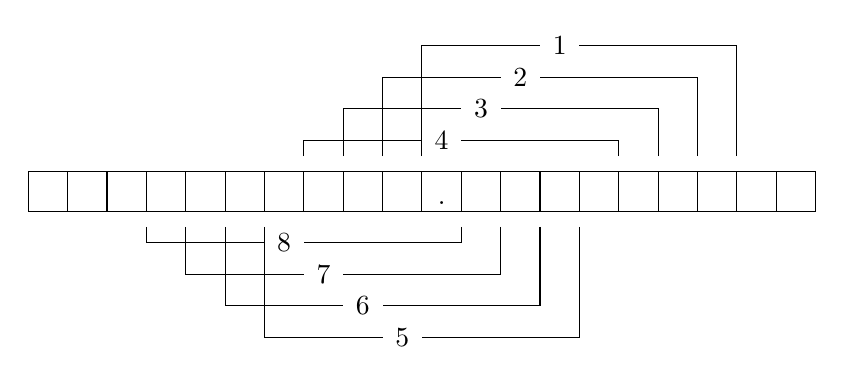
\begin{tikzpicture}
                \draw [step = 0.5] (0, 0) grid (10, 0.5);
                \node at (5.25, 0.1) {.};

                \draw (1.5, -0.2) -- (1.5, -0.4) -- (3, -0.4);
                \draw (5.5, -0.2) -- (5.5, -0.4) -- (3.5, -0.4);
                \node at (3.25, -0.4) {8};

                \draw (2, -0.2) -- (2, -0.8) -- (3.5, -0.8);
                \draw (6, -0.2) -- (6, -0.8) -- (4, -0.8);
                \node at (3.75, -0.8) {7};

                \draw (2.5, -0.2) -- (2.5, -1.2) -- (4, -1.2);
                \draw (6.5, -0.2) -- (6.5, -1.2) -- (4.5, -1.2);
                \node at (4.25, -1.2) {6};

                \draw (3, -0.2) -- (3, -1.6) -- (4.5, -1.6);
                \draw (7, -0.2) -- (7, -1.6) -- (5, -1.6);
                \node at (4.75, -1.6) {5};

                \draw (3.5, 0.7) -- (3.5, 0.9) -- (5, 0.9);
                \draw (7.5, 0.7) -- (7.5, 0.9) -- (5.5, 0.9);
                \node at (5.25, 0.9) {4};

                \draw (4, 0.7) -- (4, 1.3) -- (5.5, 1.3);
                \draw (8, 0.7) -- (8, 1.3) -- (6, 1.3);
                \node at (5.75, 1.3) {3};

                \draw (4.5, 0.7) -- (4.5, 1.7) -- (6, 1.7);
                \draw (8.5, 0.7) -- (8.5, 1.7) -- (6.5, 1.7);
                \node at (6.25, 1.7) {2};

                \draw (5, 0.7) -- (5, 2.1) -- (6.5, 2.1);
                \draw (9, 0.7) -- (9, 2.1) -- (7, 2.1);
                \node at (6.75, 2.1) {1};
            \end{tikzpicture}
            \caption{存储位的位置}
            \label{fig:NumberSystemBasics/FixedPointAndFloatingPoint/FixedPoint/Position}
        \end{figure}

        如果固定小数点的位置,那么我们便无法灵活地控制表达范围与精度。那么我们能否找到一种方式,可以让小数点的位置根据我们的数值的大小动起来,就此根据需要灵活地控制精度与表达范围呢?

    \subsection{浮点数}\label{subsec:NumberSystemBasics/FixedPointAndFloatingPoint/FloatingPoint}
        在记录小数时,为了解决定点数的缺点,我们希望
        \begin{enumerate}
            \item 能表达的数的范围要大一点;
            \item 相对精度的数量级保持平衡。一个浅显的例子是,对于几千万上亿的数字,我们所期望的绝对精度必然不会跟零点零零几的一致,前者相差几十上百没有太大影响,而后者哪怕只是相差零点一都会造成核爆般的震动,因此我们并不需要保持绝对精度,我们只需要保持与这个数的数量级相符的“相对”精度。
        \end{enumerate}

        基于这两个要求,我们可以在经过思考后发现,科学记数法(Scientific Notation)的思想似乎符合我们的愿望。

        在平时,在遇到很大或者很小的数时候,我们通常使用科学记数法来描述这个数,以避免数 $0$ 的烦恼。科学记数法使用形如 $a \times 10^b$ 的形式来记录一个数,并限定 $1 \leqslant a < 10 $,$b$ 为整数。例如,数 $16000$ 可以用科学记数法记为
        \[1.6 \times 10^4\]
        ,其中 $\times$ 号前面的尾数(Mantissa)$a$ 记录了原本的数字,后面是一个乘方的形式,其中乘方的底数事实上指示了原数的进制,称为基(Base),乘方的指数(Exponent)指示了小数点的偏移。

        这种记数法符合我们的愿望的理由是:
        \begin{enumerate}
            \item 能表达的数的范围要大一点:是的。科学记数法本就是为表达较大的数与较小的数而诞生的,要表达很大或者很小的数只需要修改指数即可,而不需要浪费非常大的空间来写 $0$,将 $0$ 写在指数部分带来的表达范围的扩增比写在尾数部分大得多了。
            \item 相对精度的数量级保持平衡:是的。乘方的形式无形中将相对精度的位置进行了适当的调整。例如,如果限制尾数保留小数点后三位,那么对于十亿一百万 $1.001 \times 10^9$ 来说,能够波动的最小误差是 $0.001 \times 10^9$ 即一百万,而对于零点零零一零零一 $1.001 \times 10^{-3}$ 来说,能够波动的最小误差是 $0.001 \times 10^{-3}$ 即百万分之一,不论原数的大小其最小误差均为原数数量级的千分之一,相对来说保持了平衡。
        \end{enumerate}

        由此,我们确认借鉴科学记数法可以解决小数的二进制记录的问题。

        在不加限制地使用这种记数法时,小数点在整个数中的相对位置是可以变化的,例如 $16000$ 和 $1.6 \times 10^4$ 与 $16 \times 10^3$ 甚至 $0.0016 \times 10^7$ 都表示同一个数,因此使用了类似于科学记数法记录的二进制小数得名“浮点数”(Floating Point Number)。
        为了保证相同数字的表示形式的唯一性,我们借鉴科学记数法的定义,将尾数 $a$ 满足 $1 \leqslant a < 10$ 的形式的表示形式指定为规格化(Normalized)\footnote{另有“规范化”、“规约化”、“规则化”、“正规化”等翻译。}数,其他的称为非规格化(Denormalized)数。

        由于现代通用的计算机均使用二进制,因此我们借鉴来的记录方式应该使用(十进制表示的)$a \times 2^b$,而且因为基固定为 $2$ 因此可以省略,于是我们只需要记录 $a$ 和 $b$ 便可以记录这个数。并且,如果确保记录的浮点数必定为规格化数的话,二进制表示的 $b$ 必定是 $\overline{1.b_1b_2 \cdots b_n}$ 的以 $1$ 开头的形式,因此 $b$ 开头的 $1$ 也可以省略。

        当然,在我们使用相同的长度来表达一个小数的时候,定点数可以完全使用这一段长度来记录它,但浮点数需要在这段有限的长度中抠出一部分用于保存指数信息,这会损失一定的精度。但是,我们一方面以此换来了更大的数值范围,而且只要权衡好抠出的量的话损失少量的精度在大部分情况下是可以接受的。
